%%%%%%%%%%%%%%%%%%%%%%%%%%%%%%%%%%%%%%%%%%%%%%%%%%%%%%%%%%%%%%%%%%%%%%%%%%%%%%%%
%2345678901234567890123456789012345678901234567890123456789012345678901234567890
%        1         2         3         4         5         6         7         8
% THESIS Chapter

\chapter{Background theory}
\label{chap:relatedterms}
\ifpdf
    \graphicspath{{RelatedTerminology/Figures/PNG/}{RelatedTerminology/Figures/PDF/}{RelatedTerminology/Figures/}}
\else
    \graphicspath{{RelatedTerminology/Figures/EPS/}{RelatedTerminology/Figures/}}
\fi


% short summary of the chapter `` ''
% \section*{Summary}

% Describe here the state of the art of the research pertaining to this thesis. This part should contain all the relevant publications in the area with the corresponding citations. The cited works should be briefly described critically assessed.
%

Each type of information extracted from an audio stream is referred to as an
\textit{audio feature}. Audio features are mainly derived using various 
transformations on the signal based on some basic properties of sound. This
section presents low-level theory required to understand the high-level
description of how each feature is obtained further in the report.


\section{Basic properties of audio signal}
\label{sec:audioprops}
A \textit{digital audio signal} is a representation of the continuous sound wave
as a series of binary numbers. This representation helps preserve the
\textit{frequency} (the speed of the vibrations), as well as the
\textit{amplitude} (the fluctuations of the vibrations) of the sound. The energy
that each sound wave emits through vibrations is called \textit{sound energy}
and its rate is measured through \textit{sound power}. The majority of audio
features use frequency or power as a primary audio property used to define the
feature (\textit{modify/change}). 

The process of converting an analogue sound wave to a digital one involves a
process of extracting points (samples) from the continuous signal and using them
to describe the signal into a discrete form. This method is called
\textit{sampling} and the amount of samples collected per time frame is
\textit{sample rate}. The representation of a song used during feature
extraction is a sequence of samples extracted from the digital signal of the
song based on its sample rate.

\paragraph{}
In order to understand how properties of a digital signal could form audio
features we first need to examine how they relate to the ways of how people
perceive music and sound. Western music is described using \textit{tones},
steady periodic sounds \cite{wiki:tone}. They can be pure if the sound has
sinusoidal waveform, or complex if they are a combination of pure tones with a
periodic repetition pattern. A half tone is called a \textit{semitone} and it is
the smallest measure of period between sounds. Semitones are grouped into
\textit{octaves} where each octave contains 12 semitones. The acoustic opposite
of tone is noise, a disordered sound which is unpleasant to the human brain and
is disruptive to hearing \cite{music-noise}.

Tones are distinguished by several basic perceptual properties of sound - pitch,
loudness, timbre and duration \cite{acoustic-glossary-power}. Consequently these
properties are also regularly used to describe what is accurately captured by
each audio feature. Klapuri et al. \cite{klapuri2007signal} form good
definitions of the psychoacoustical terms outlined. They define \textit{pitch}
as a perceptual attribute which offers ordering of tones on a
frequency-related scale. Different pitches could be labelled through the
Helmholz pitch notation \cite{helmholtz2013sensations} using letters, through
scientific pitch notation \cite{fletcher1934loudness} utilising letters and
numbers, or directly using numbers representing the closest frequency in hertz
(hz). Despite being determined by clear and stable frequencies in sound, pitch
is more importantly a subjective auditory sensation, so a strict mathematical
relationship between frequency and pitch does not exist
\cite{acoustical1986american}. As a standard it is accepted the musical note of
A above C (Helmholz notation) or A4 (scientific notation) has a frequency of 440
Hz \cite{young1939terminology}. The human ear perceives musical intervals on an
approximately logarithmic scale with respect to a \textit{fundamental
frequency}, the lowest frequency available in a tone and therefore determining
the overall pitch of the tone. Using this notion of logarithmic perception there
are various mappings of pitches to frequencies, the most famous of which is the
MIDI tuning standard \cite{mts}.

\textit{Loudness} is another subjective psychoacoustical attribute of sound
\cite{klapuri2007signal}. Similar to how pitch is related to frequency, loudness
is a perception of sound pressure. \textit{Sound pressure} is a measurement of
the pressure divergence caused by a sound wave to the ambient atmospheric
pressure \cite{sound-pressure}. Loudness orders sounds on a scale ranging from
quiet to loud \cite{acoustical1986american}.

Tones also have a "colour" attribute attached to them through the introduction
of \textit{timbre}. Timbre allows distinguishing sounds with potentially
identical pitch, loudness and duration, but produced by different musical
instruments \cite{klapuri2007signal}. It is a complex concept which cannot be
defined by a single property of sound. There are many attempts at breaking down
the attribute into components. Robert Erickson \cite{erickson1975sound} offers
one of the most accepted decompositions where timbre relates to the following
acoustic parameters of sound:
\begin{enumerate}
    \item Tonal and noise characters
    \item Time envelope - A \textit{time envelope} describes how sounds changes
    over time \cite{wiki:envelope}. It measures how much time it takes for the sound to reach an
    amplitude level when a musical instrument is activated (a key on the piano
    is pressed, for example) and subsequently how long it takes for the sound to
    go back to its initial level. 
    \item Spectral envelope and any changes to it - when only the curve of the
    amplitude out of a time envelope is taken into consideration then a
    \textit{spectral envelope} is used. Figures \ref{fig:time-envelope} and
    \ref{fig:spectral-envelope} illustrate the difference of between both envelopes.
    \item Changes in the fundamental frequency
    \item Onset dissimilar to the dominant vibration - with \textit{onset}
    signifying the start of a musical note we look for 'anomalies' in
    the vibration of the wave compared to the vibrations following the anomaly.

\end{enumerate}

\begin{figure}
    \centering
    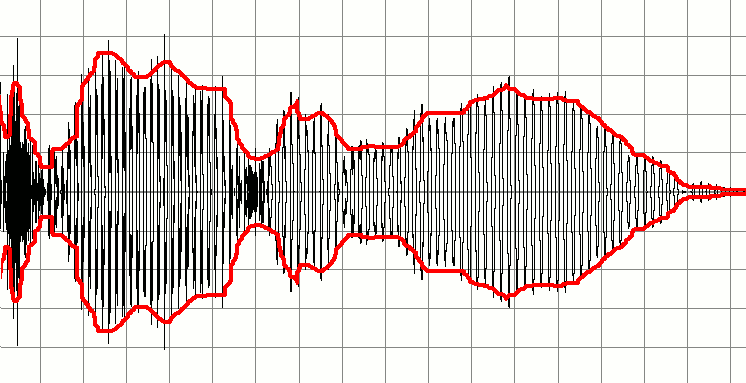
\includegraphics[width=0.75\textwidth]{BackgroundTheory/time_envelope.png}
    \captionof{figure}{Time envelope}
    \label{fig:time-envelope}
\end{figure}

\begin{figure}
    \centering
    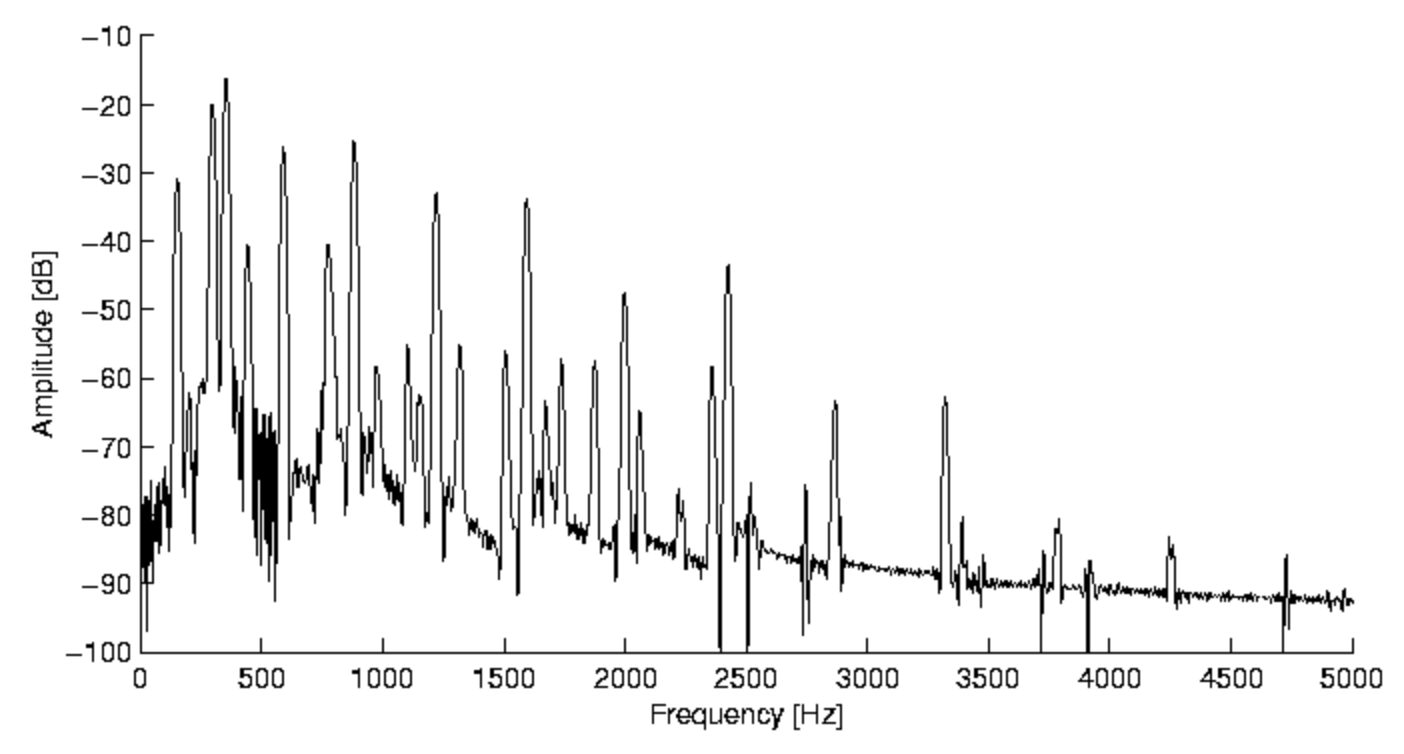
\includegraphics[width=0.75\textwidth]{BackgroundTheory/spectral_envelope}
    \captionof{figure}{Spectral envelope}
    \label{fig:spectral-envelope}
\end{figure}

ADD \textit{duration}

%  Connect the signal-based properties of sound with the musical ones - explain
% pitch, octave, beat and beat onset, timbre, loudness


\subsection{Test subsection}
\label{sec:subsec21}

\section{Audio transformation techniques}
Explain spectrum first - we use a spectrum of a basic property to determine an
audio feature
mention frequency spectrum for example - make the analogy with determining
loudness by projecting spl over the frequency spectrum
then fourier transform
MENTION THAT THE FUNDAMENTAL FREQUENCY DETERMINES THE PITCH OF TONE BECAUSE IT
IS THE COMMON DENOMINATOR FREQUENCY OF ALL COMPRISING FREQUENCIES

\label{sec:audiotransform}
% add more sections and subsection here
